\title{Модульная архитектура проекта YaccConstructor на основе Mono.Addins}
%
\titlerunning{Модульная архитектура проекта YaccConstructor}

\author{Орлов Илья Денисович}
%
\authorrunning{И.Д.Орлов} % abbreviated author list (for running head)
%
%%%% list of authors for the TOC (use if author list has to be modified)
\tocauthor{И.Д.Орлов}
%
\institute{Санкт-Петербургский государственный университет\\
\email{2x2.4raymon@gmail.com}}

\maketitle

\begin{abstract}
Большинство  достаточно  крупных проектов разбиты на части, называемые
модулями.     Для    функционирования    проекта  в целом   необходимо
поддерживать    корректное    взаимодействие   между   модулями.   Для
задач  такого  типа  существуют  готовые  инструменты.  Данная  работа
посвящена Mono.Addins, одному из таких инструментов, его достоинствам,
а также применению данного инструмента в проекте YaccConstructor.
\end{abstract}

% У введения нет номера главы
\section*{Введение}
При разработке проекта приходится часто изменять какие-либо его части: что-то улучшать, корректировать, добавлять, менять версии. При таких действиях возникает проблема согласованности разных частей проекта. Сможет ли какая-то часть работать корректно, если произведены изменения в другой? Для удобства таких манипуляций хочется сделать части проекта максимально независимыми друг от друга. Чтобы функциональность одной как можно меньше зависела от реализации другой. То есть хочется разбить проект на отдельные независимы подпрограммы, называемые модулями, которые предоставляют друг другу лишь какой-то интерфейс, при этом не вдаваясь в реализацию.

Принцип, при котором проект разбит на отдельные компоненты (модули) называется модульностью. Такая организация проекта имеет существенные достоинства перед той, у которой части проекта тесно связаны друг с другом. Модульность упрощает задачи разработки проекта и распределения процесса работы между группами разработчиков. Таким образом возникает меньше простоев в работе команды на проектом в целом. А также меньше сбоев и конфликтных ситуаций при написании кода. Существенным достоинством также является возможность локализации ошибок в проекте в целом и уменьшение времени компиляции.

Простым примером может являться следующая схема:

\begin{figure}[h!]
\begin{center}
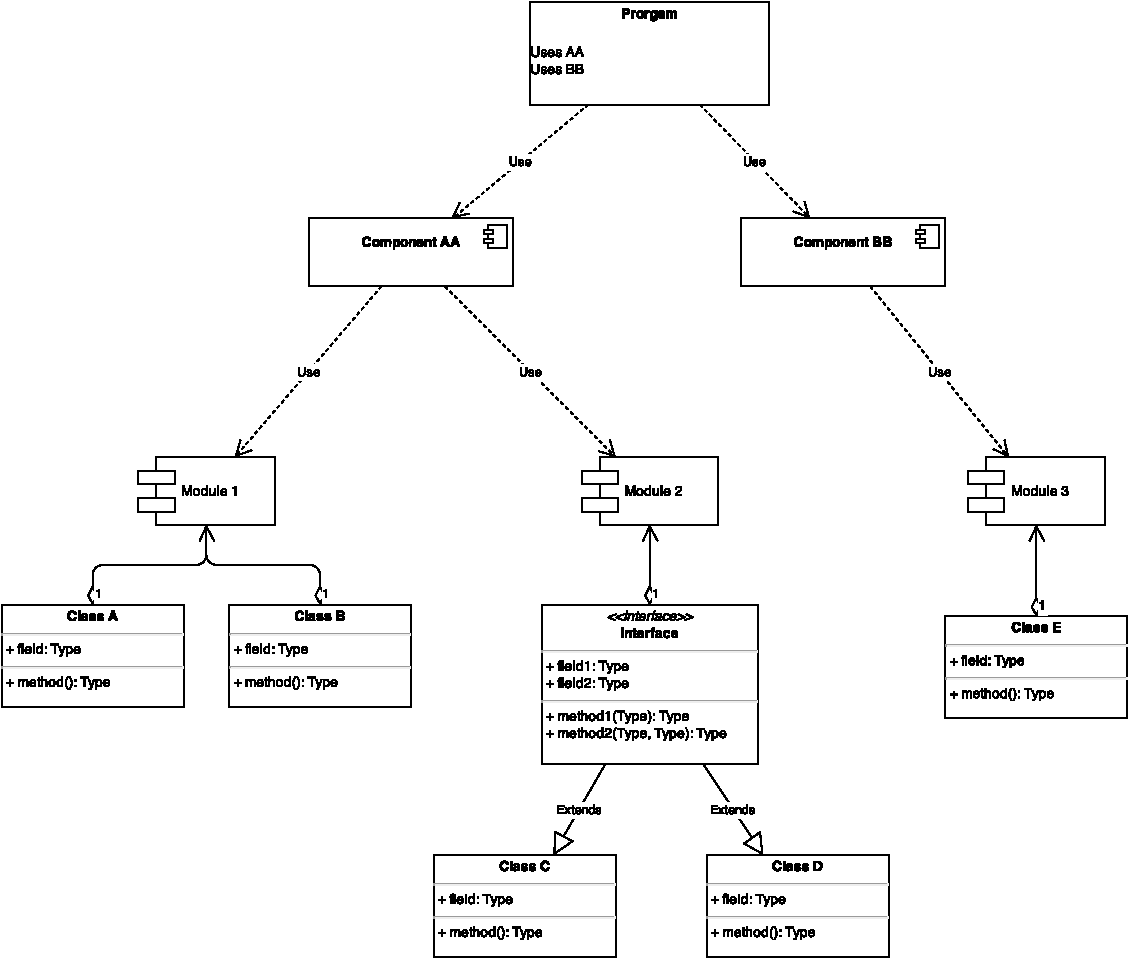
\includegraphics[width=\linewidth]{Orlov/module_example}
\caption{Пример модульной иерархии}
\label{fig:module_example} 
\end{center}
\end{figure}

Модули 1,2 и 3 являются независимыми друг от друга по реализации, при этом в программе используется функциональность каждого из них.

Простым примером также является подключение плагина к какой-нибудь среде разработки. Нет необходимости разбираться в устройстве самой среды. Достаточно воспользоваться предоставляемым интерфейсом (прописать нужные пути, положить плагин в нужную директорию) для интеграции плагина.

Для организации модульной структуры необходимо реализовать каждый модуль по отдельности, а также те компоненты проекта, которые будут отвечать за связь между модулями. На данный момент существует некоторые готовые инструменты, позволяющие не реализовывать свою поддержку модульности, а обеспечить ее через предоставляемый инструментом интерфейс.
Таки образом целью работы является реализация модульности через имеющийся инструмент Mono.Addins в проекте YaccConstructor.

\section{Постановка задачи}
В рамках данной работы были поставлены следующие задачи:
\begin{itemize}
\item Удаление компонент, отвечающих за собственную поддержку модульности
\item Реализация поддержки модульности на основе существующего инструмента Mono.Addins
\item Реализация тестов под новый инструмент
% \item Сравнение скоростей загрузки компонент
\end{itemize}

\section{Обзор}
Для реализации модульности в проекте существует инструмент Mono.Addins\footnote{http://monoaddins.codeplex.com}.
Инструмент имеет следующие достоинства\footnote{http://mono-project.com/Introduction\_to\_Mono.Addins}:
\begin{itemize}
\item Поддержка метаданных, что позволяет хранить метаданные к готовой компоненте (модулю)
\item Поддержка иерархии модулей. Mono.Addins умеет загружать модули (по рефлексии), которые в свою очередь зависят от других компонент
\item Поддержка описания надстроек (модулей) позволяет описывать надстройки, используя или пользовательские атрибуты, или XML файлы (для более сложных компонент)
\item «Ленивая» загрузка модулей. Mono.Addins загружает только те модули, которые необходимы в данный момент
\item Динамическая загрузка модулей. Загрузка модулей происходит при исполнении программы. Также можно отключать некоторые компоненты во время исполнения
\end{itemize}

Также Mono.Addins поддерживается проектами, написанными под .NET, и устанавливается из репозитория, что удобно для использования в проекте YaccConstructor.

YaccConstructor – проект по разработке средств реинжиниринга\footnote{https://code.google.com/p/recursive-ascent}. Представляет собой инструмент для лексического анализа и синтаксического разбора~\cite{YC_base}.  Структура проекта состоит из трех основных компонент, которые видно на следующем рисунке:

\begin{figure}[h!]
\begin{center}
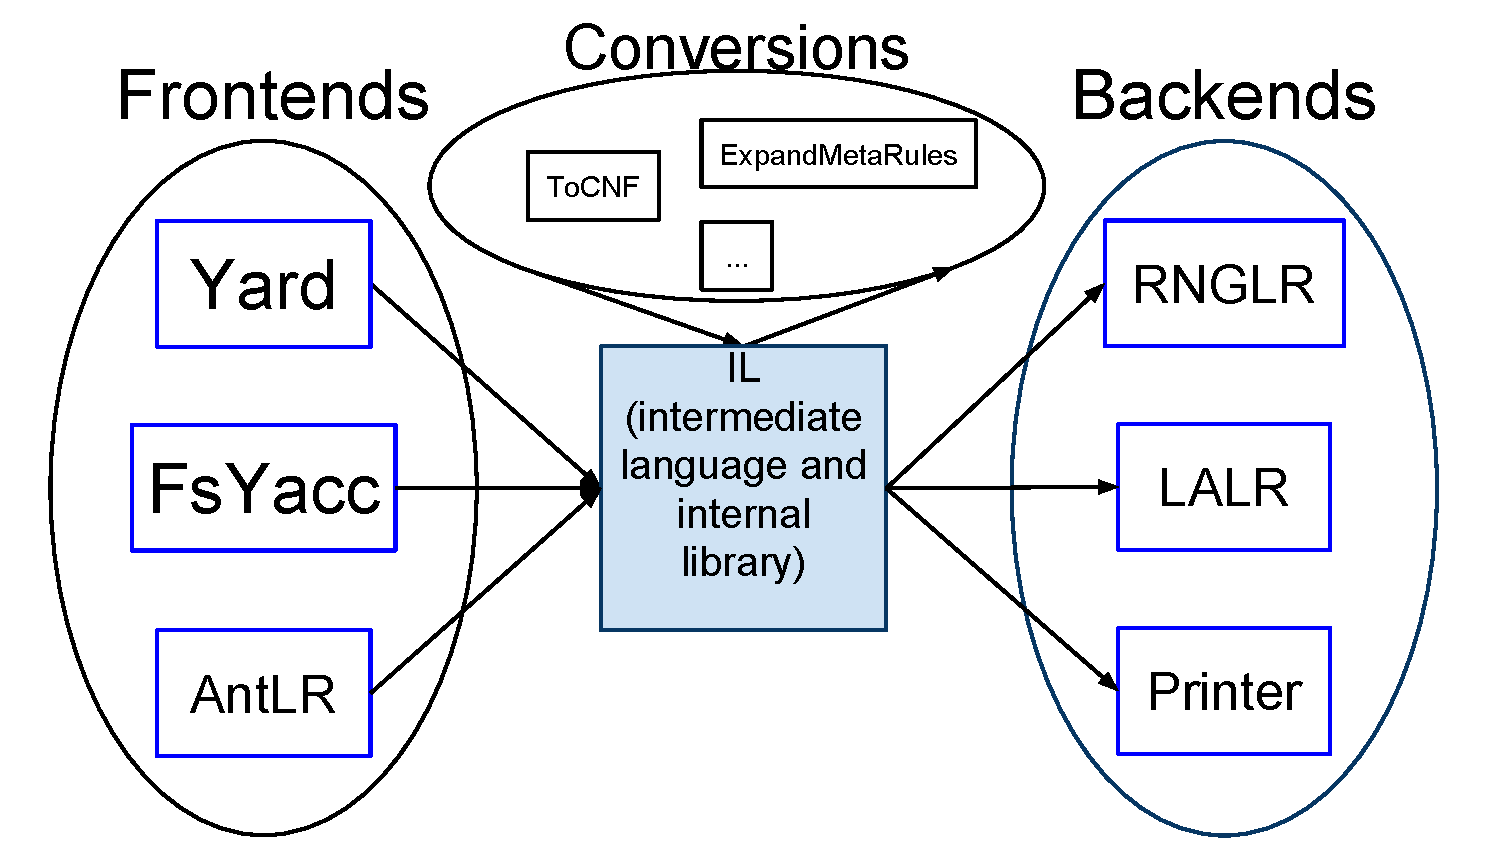
\includegraphics[width=\linewidth]{Orlov/structyc}
\caption{Ирерархия проекта YaccConstructor}
\label{fig:structyc} 
\end{center}
\end{figure}

Сами компоненты~\cite{YC_article}:
\begin{itemize}
\item Фронтенды --- модули, которые по грамматике на конкретном языке создают IL, так называемый некий промежуточный язык (генерируется в виде дерева), который обрабатывается генератороми
\item Соглашения  --- часть проекта, которая добавляет некоторые соглашения в уже сгенерированный IL
\item Генераторы --- модули, которые по промежуточному языку генерируют код на F\#
\end{itemize}

Каждая компонента состоит из модулей, которые содержат конкретные реализации фронтендов, соглашений и генераторов.

Как можно заметить, компоненты проекта и модули являются достаточно независимыми друг от друга по реализации. Каждая из компонент предоставляет другой на вход лишь некоторые данные, при этом не вдаваясь в функциональность. Можно написать еще один фронтенд и  включить его в проект, не нарушив тем самым работоспособность других модулей или компонент.

В проекте уже была реализована своя поддержка модульности. Во время исполнения программы пользователь сам выбирает, каким именно фронтендом и генератором он хочет пользоваться. Решение о реализации своей поддержки модульности являлось правильным на тот момент, так как не существовало готовых инструментов. Более правильным же является использование готовых компонент, если такие имеются, так как это существенно сокращает имеющийся код и загружает модули более аккуратно, не теряя при этом свойств загрузки.



\section{Реализация}
\subsection {Удаление компонент, отвечающих за собственную \\поддержку модульности}
Основными компонентами, отвечающими за поддержку модульности, являются те, которые обеспечивают взаимодействие компонент друг с другом и подгружают необходимые модули во время исполнения.
В проекте YaccConstructor на каждую компоненту (фронтенды, соглашения, генераторы) был реализован свой собственный загрузчик (менеджер), который умел составлять список конкретно реализованных модулей и выдавать его в программе. Также существовал общий менеджер --- абстрактный интерфейс для реализации каждого отдельного менеджера компонент.

\begin{figure}[h!]
\begin{center}
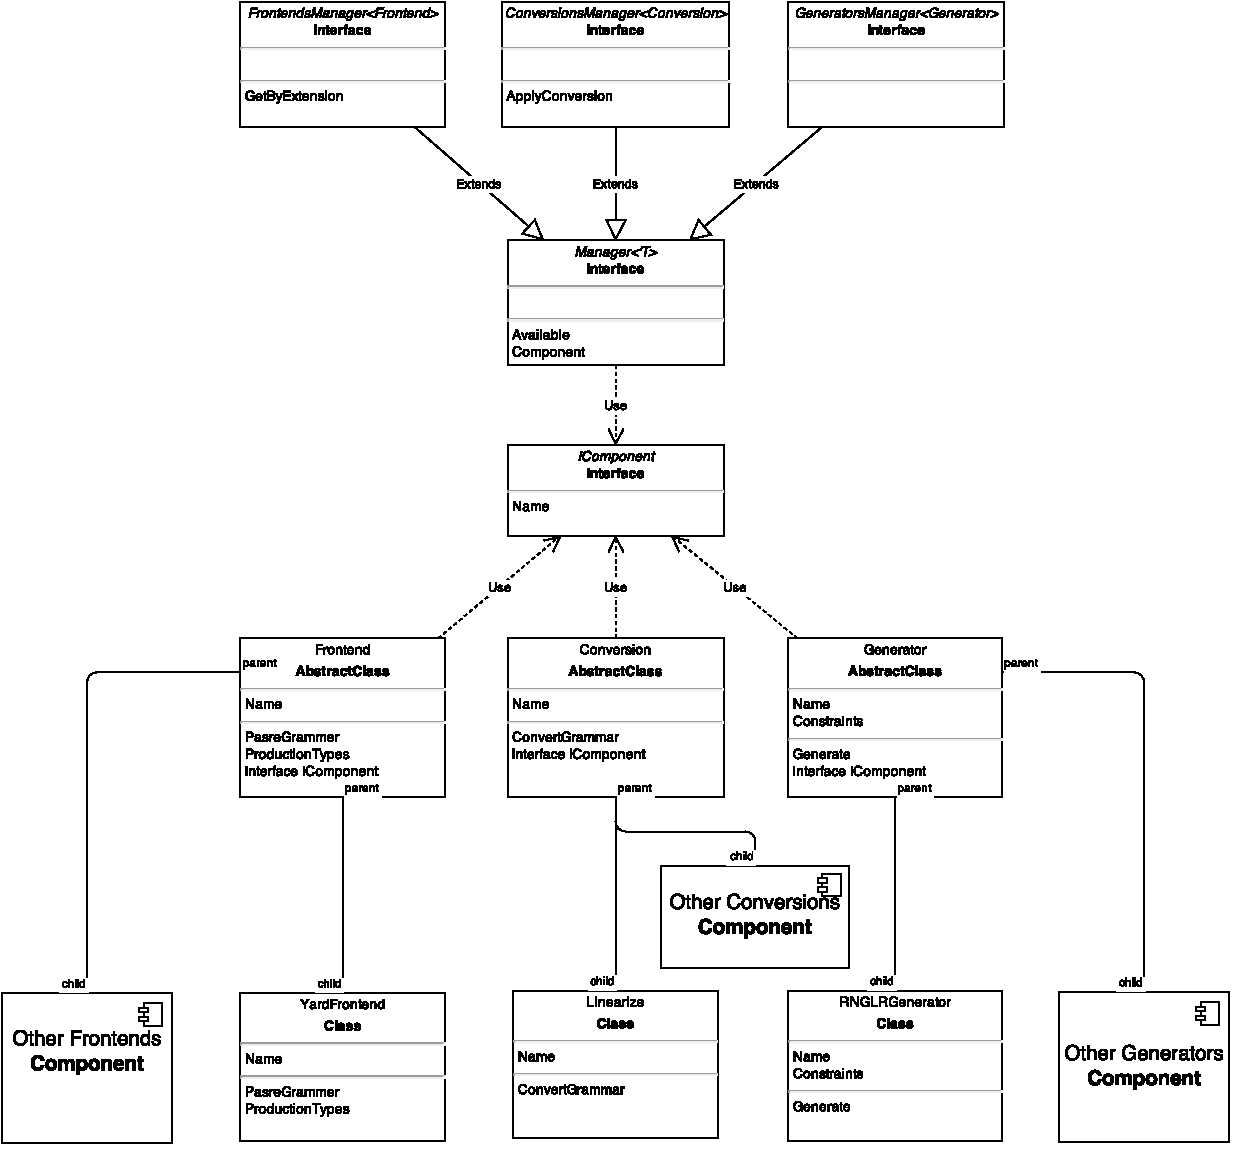
\includegraphics[width=\linewidth]{Orlov/yc_was}
\caption{Компоненты проекта YaccConstructor. Реализация своей поддержки модульности}
\label{fig:yc_was} 
\end{center}
\end{figure}

Общий менеджер находится в центре диаграммы. Сверху располагаются менеджеры для загрузки отдельных компонент. Они унаследованы от основного менеджера. Загрузчики используют интерфейс IComponent, который предоставляет имя каждого конкретного модуля при реализации. А также метод Available, который предоставляет загрузчику конкретные модули. В нижней части диаграммы видно иерархию самих основных компонент проекта, которые также используют интерфейс  IComponent. Для избавления от своей поддержки модульности были полностью удалены все менеджеры, а также интерфейс IComponent.

\subsection {Реализация поддержки модульности на основе \\Mono.Addins}.
Вместо интерфейса IComponent у каждого модуля появилось обычное поле с названием. Далее необходимо было собрать все имеющиеся компоненты и модули в менеджеры, которые предоставляет Mono.Addins. 
Для включения компоненты или модуля в менеджер загрузки имеются следующие атрибуты:
\begin{itemize}
\item TypeExtensionPoint --- атрибут, которым помечается интерфейс или абстрактный класс компоненты.
\item Extension --- атрибут, которым помечается непосредственная реализация какого-либо модуля.
\end{itemize}

В проекте YaccConstructor реализация выглядит следующим образом:
\begin{figure}[h!]
\begin{center}
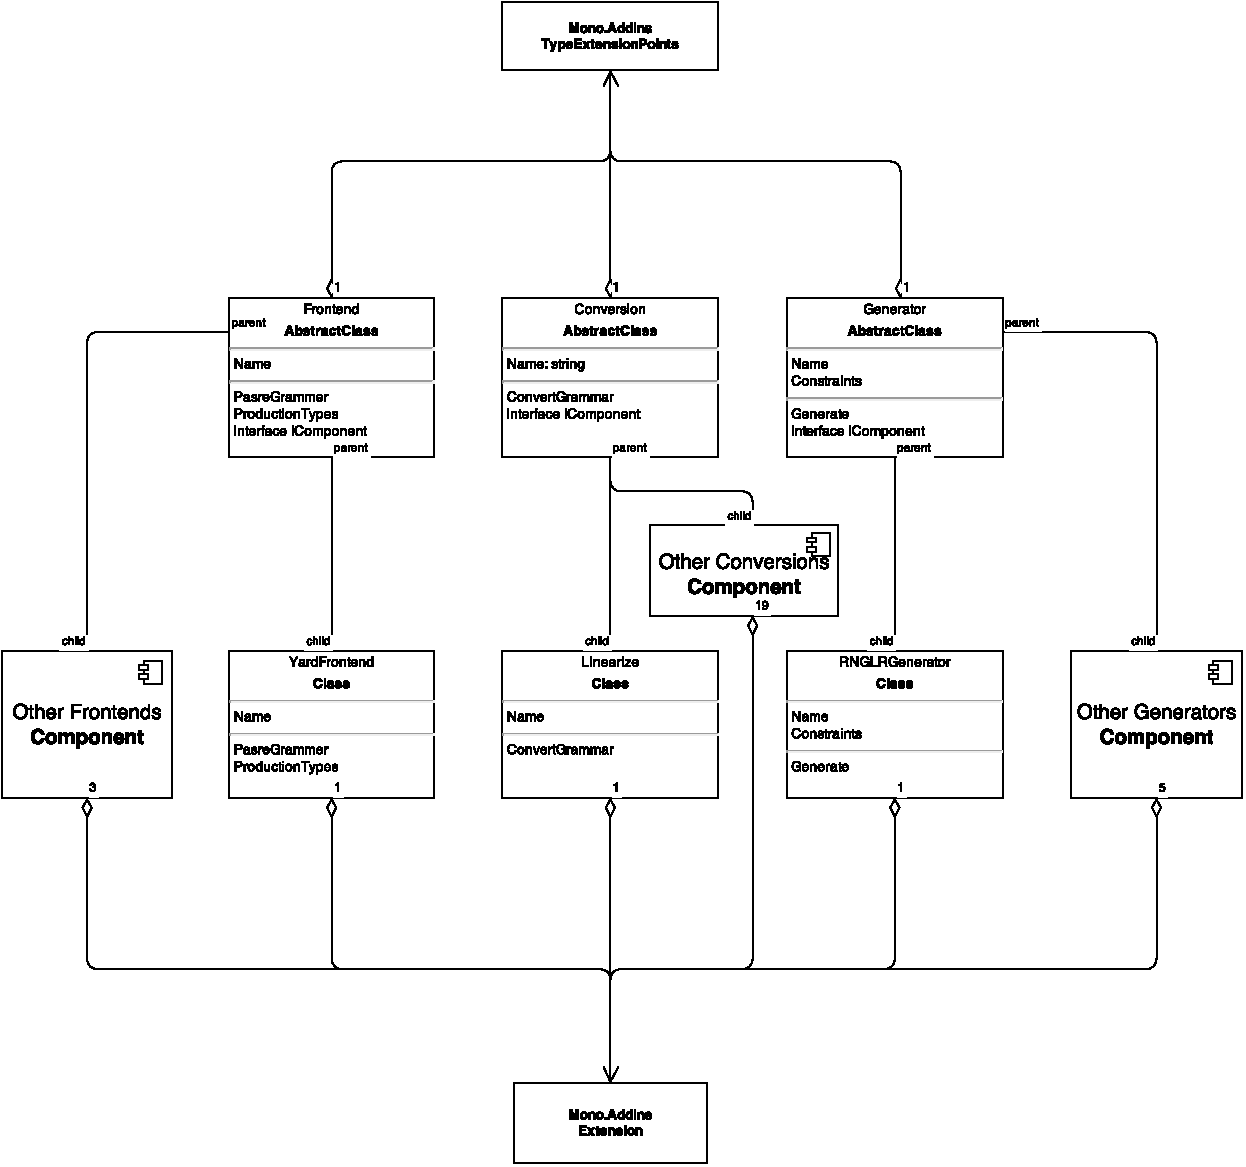
\includegraphics[width=\linewidth]{Orlov/yc_now}
\caption{Компоненты проекта YaccConstructor. Реализация поддержки модульности на основе Mono.Addins}
\label{fig:yc_now} 
\end{center}
\end{figure}

В верхней части диаграммы располагаются абстрактные классы фронтендов, соглашений и генераторов, которые помечаются атрибутом TypeExtensionPoint.
В нижней части располагаются непосредственные реализации модулей, которые помечаются атрибутом Extension.

Примеры использования атрибутов:
\begin{itemize}
\item  Таким образом можно, например, создать новую абстрактную компоненту в проекте и включить ее в Mono.Addins --- пример использования атрибута TypeExtensionPoint:
\begin{verbatim}
 [<assembly:AddinRoot ("YaccConstructor", "1.0")>]
 do()
 
 [<AbstractClass>]
 [<TypeExtensionPoint>]
    type Generator() as this = 
        methods
\end{verbatim}


\item Таким образом можно подключить новый реализованный модуль, который наследуется от абстрактного интерфейса --- пример использования атрибута Extension: 

\begin{verbatim}
 [<assembly:Addin>]
 [<assembly:AddinDependency ("YaccConstructor", "1.0")>]
 do()
 
 [<Extension>]
 type RNGLR() =
    inherit Generator()
        realization
\end{verbatim}
\end{itemize}

Таким образом в исполняемом модуле программы имеем менеджеры, предоставляемые Mono.Addins, содержащие реализации конкретных компонент. По ним был реализован поиск нужного генератора или фронтенда, а также простой вывод всех доступных на данный момент модулей в целом. Можно видеть из диаграмм \ref{fig:yc_was} и \ref{fig:yc_now}, что структура проекта стала проще, поскольку число самих компонент уменьшилось. Также стало проще работать с уже реализованными  модулями, поскольку стало меньше зависимостей от других интерфейсов.
При этом общее количество кода сократилось примерно на 200 строк, что составляет 5 файлов.

\subsection {Реализация тестов под новый инструмент}

Как и любой другой проект YaccConstructor содержит тесты на проверку корректности работы компонент.
Однако эти тесты были зависимыми от тех менеджеров, которые были реализованы в своей поддержки модульности. Для этого тесты были пересмотрены с учетом новых менеджеров, предоставляемых Mono.Addins. Также были вынесены дополнительные функции, которые содержались в методах старых загрузчиков.


\section*{Заключение}
В ходе данной работы были получены следующие результаты:
\begin{itemize}
\item Изучен инструмент Mono.Addins.
\item Удалена своя поддержка модульности в проекте  YaccConstructor.
\item Реализована поддержка модульности в проекте YaccConstructor на основе Mono.Addins.
\item Пересмотрены тесты под новую поддержку модульности.
% \item Проведены замеры времени работы различных реализаций модульности
\end{itemize}

\begin{thebibliography}{99}
\bibitem{YC_base}
Я.А.Кириленко, С.В.Григорьев, Д.А.Авдюхин. 
Разработка синтаксических анализаторов в проектах по автоматизированному реинжинирингу информационных систем //
Научно-технические ведомости Санкт-Петербургского государственного политехнического университета. Информатика. Телекоммуникации. Управление,
2013.

\bibitem{YC_article}
А.У.Константин. Инструмент реинжиниринга спецификаций трансляций.
Дипломная работа. СПбГУ, кафедра Системного программирования, 2011.
\end{thebibliography}
